\clearpage
\section*{二、实验操作与原始数据}

\subsection*{1. 实验操作与原始记录}

实验时，我先打开变温界面张力分析仪预热，用水准泡将测试架调平，再按课堂要求设置示波器：探头比 1×，纵向增益 $200\,\mathrm{mV/DIV}$；定标时横向增益不大于 $1\,\mathrm{ms/DIV}$，拉脱时不小于 $2\,\mathrm{s/DIV}$，采用光标读数。下面两张照片是调试时的探头设置和示波器参数。

\begin{figure}[H]\centering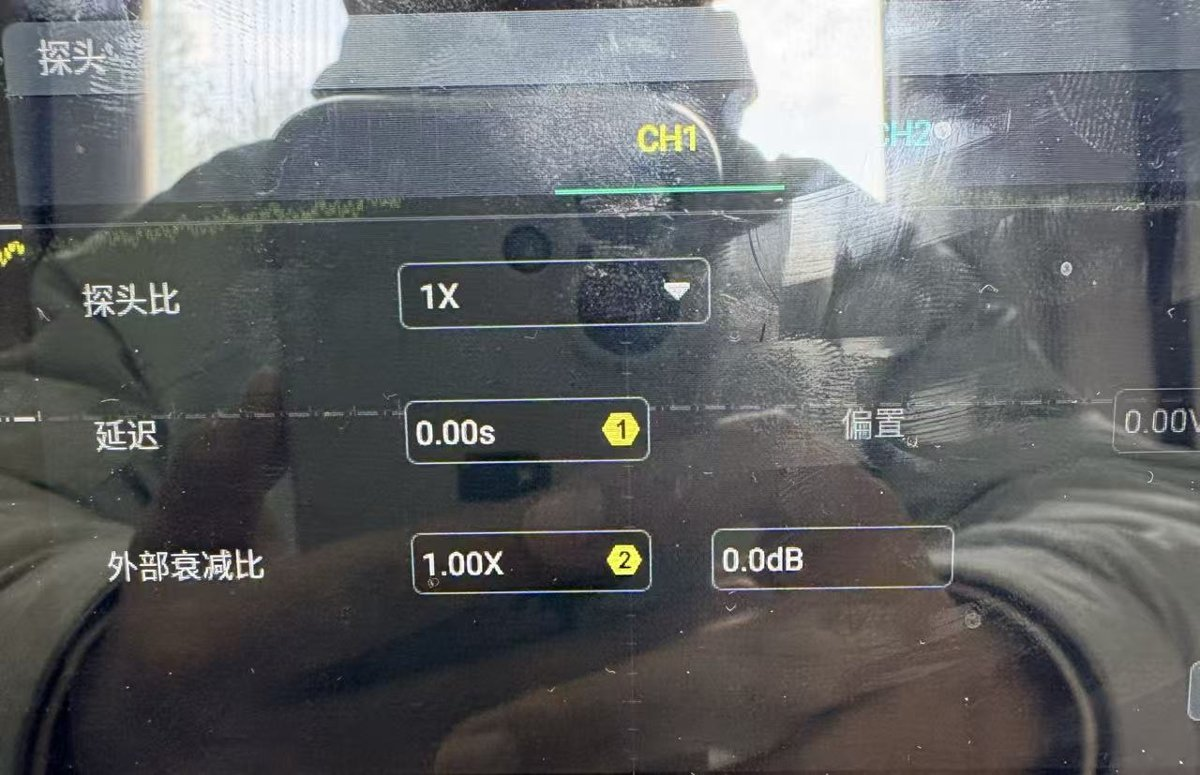
\includegraphics[width=9cm]{../assets/osc-probe.jpg}\caption{调试时的探头设置（CH1 探头比 1×）}\end{figure}

\begin{figure}[H]\centering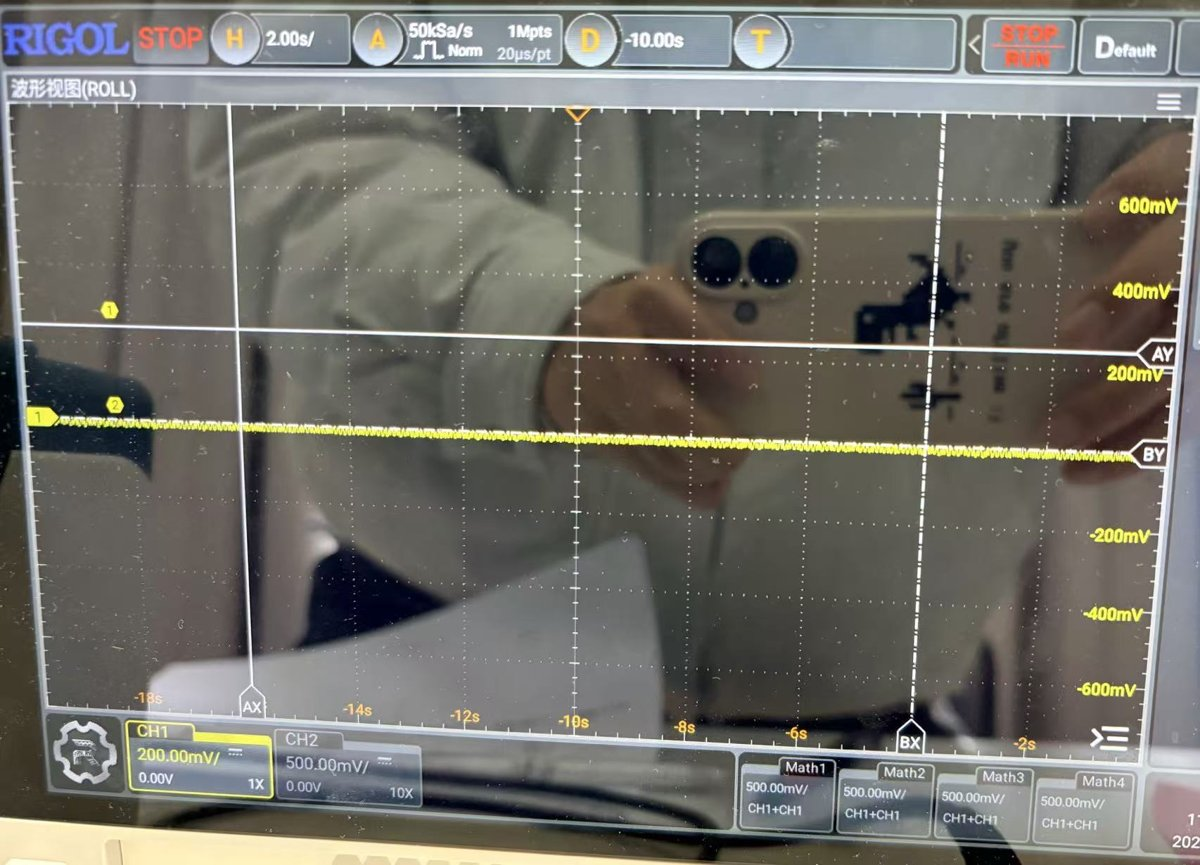
\includegraphics[width=10cm]{../assets/osc-settings.jpg}\caption{调试时的示波器参数（CH1 200 mV/DIV，时基 2.00 s/DIV，已暂停）}\end{figure}

定标时，挂上砝码盘并将拉力置零，以 $500\,\mathrm{mg}$ 为一档逐个加砝码至 $3500\,\mathrm{mg}$，再逐个减少，分别记录电压。随后取下砝码盘，用游标卡尺在不同方向各测 6 次圆环的内径 $d_1$ 和外径 $d_2$。

拉脱测量前，我挂上圆环并在初始时调零，此后圆环基线读数均记为 0。室温 $18.8\,{}^\circ\mathrm{C}$ 下测量 6 次，再将水温升至 $26\,{}^\circ\mathrm{C}$ 和 $35\,{}^\circ\mathrm{C}$，各测 6 次。原始记录如下。

\begin{figure}[H]\centering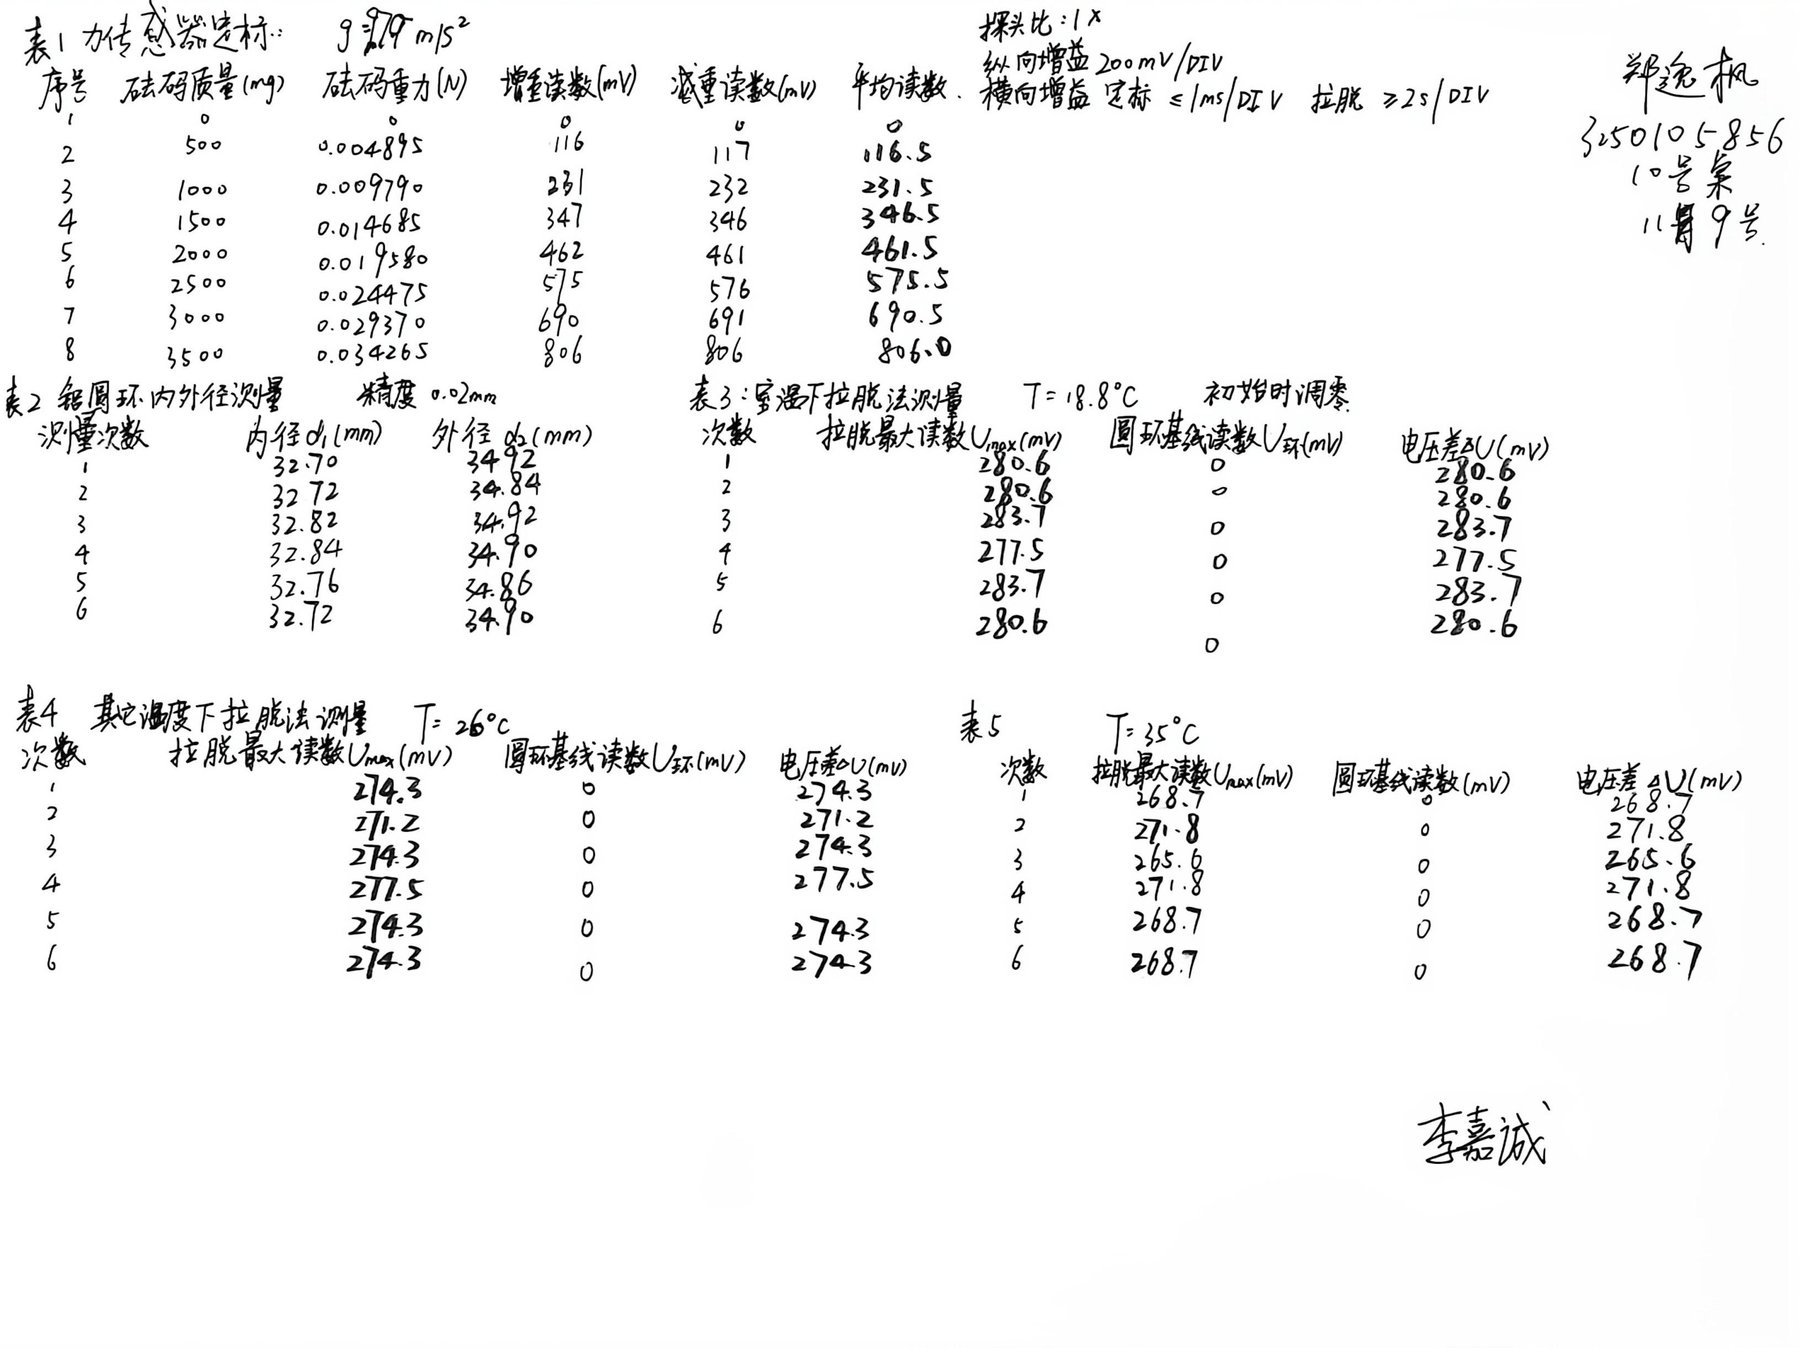
\includegraphics[width=16cm]{../assets/raw-data.jpg}\caption{本次原始记录（已按阅读方向旋转）}\end{figure}

\clearpage

\subsection*{2. 力敏传感器定标数据}

取杭州重力加速度 $g=9.79\,\mathrm{m/s^2}$，平均读数为增重与减重读数的平均值。

\begin{center}\small
\begin{tabular}{cccccc}
\toprule
序号 & 砝码质量/mg & 砝码重力/N & 增重读数/mV & 减重读数/mV & 平均读数/mV \\
\midrule
1 & 0 & 0 & 0 & 0 & 0 \\
2 & 500 & 0.004895 & 116 & 117 & 116.5 \\
3 & 1000 & 0.009790 & 231 & 232 & 231.5 \\
4 & 1500 & 0.014685 & 347 & 346 & 346.5 \\
5 & 2000 & 0.019580 & 462 & 461 & 461.5 \\
6 & 2500 & 0.024475 & 575 & 576 & 575.5 \\
7 & 3000 & 0.029370 & 690 & 691 & 690.5 \\
8 & 3500 & 0.034265 & 806 & 806 & 806.0 \\
\bottomrule\end{tabular}\end{center}

\subsection*{3. 圆环内外径}

游标卡尺分度值为 $0.02\,\mathrm{mm}$。

\begin{center}\small
\begin{tabular}{ccccccc}
\toprule
测量次数 & 1 & 2 & 3 & 4 & 5 & 6 \\
\midrule
内径 $d_1$/mm & 32.70 & 32.72 & 32.82 & 32.84 & 32.76 & 32.72 \\
外径 $d_2$/mm & 34.92 & 34.84 & 34.92 & 34.90 & 34.86 & 34.90 \\
\bottomrule\end{tabular}\end{center}

\subsection*{4. 拉脱法测量数据}

三个温度下的圆环基线读数 $U_{\text{环}}$ 均为 0，故电压差 $\Delta U=U_{\max}-U_{\text{环}}=U_{\max}$。表中为各次的 $\Delta U$，单位为 mV。

\begin{center}\small
\begin{tabular}{ccccccc}
\toprule
水温 & 1 & 2 & 3 & 4 & 5 & 6 \\
\midrule
$18.8\,{}^\circ\mathrm{C}$（室温） & 280.6 & 280.6 & 283.7 & 277.5 & 283.7 & 280.6 \\
$26\,{}^\circ\mathrm{C}$ & 274.3 & 271.2 & 274.3 & 277.5 & 274.3 & 274.3 \\
$35\,{}^\circ\mathrm{C}$ & 268.7 & 271.8 & 265.6 & 271.8 & 268.7 & 268.7 \\
\bottomrule\end{tabular}\end{center}

\clearpage

